\subsubsection{Package sequenziatore::client::iview::iprocessowner}

\paragraph{IMainProcessOwner}
\begin{figure}[H] \centering 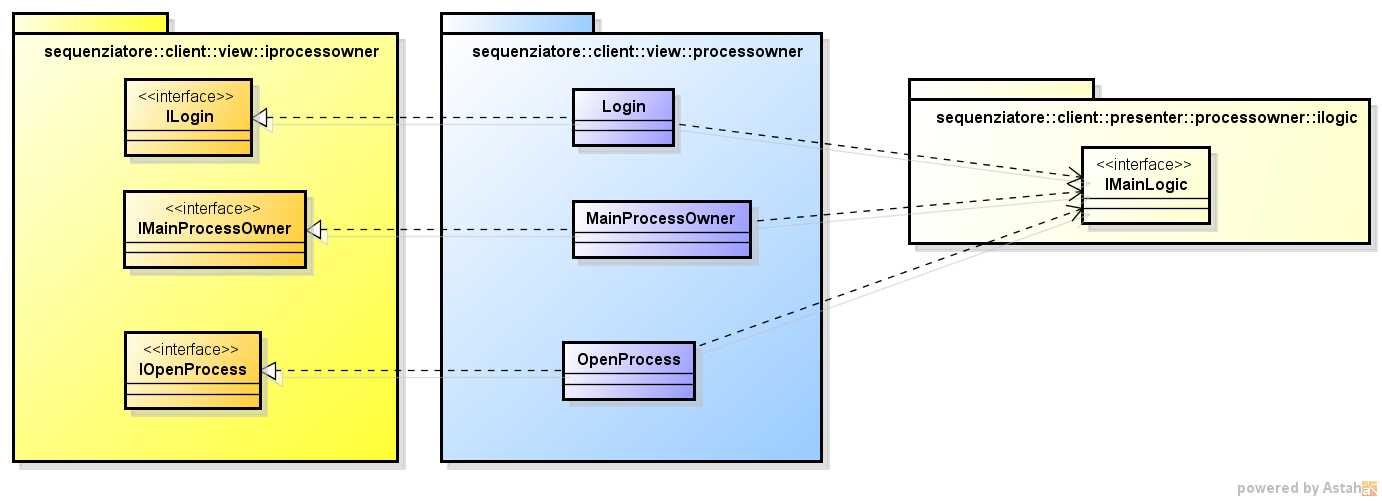
\includegraphics[width=%
\textwidth]
{./pack/ProcessOwner.png} \caption{Diagramma view principale process owner}
\end{figure}
\begin{itemize}
\item \textbf{Nome:} \texttt{IMainProcessOwner};
\item \textbf{Package:} \texttt{\iViewAdmin{}};
\item \textbf{Descrizione:} Interfaccia che permette la gestione delle principali componenti dell'interfaccia grafica dell'utente \textit{process owner\ped{G}}.
\end{itemize}

\paragraph{IUpdateView}
\begin{figure}[H] \centering 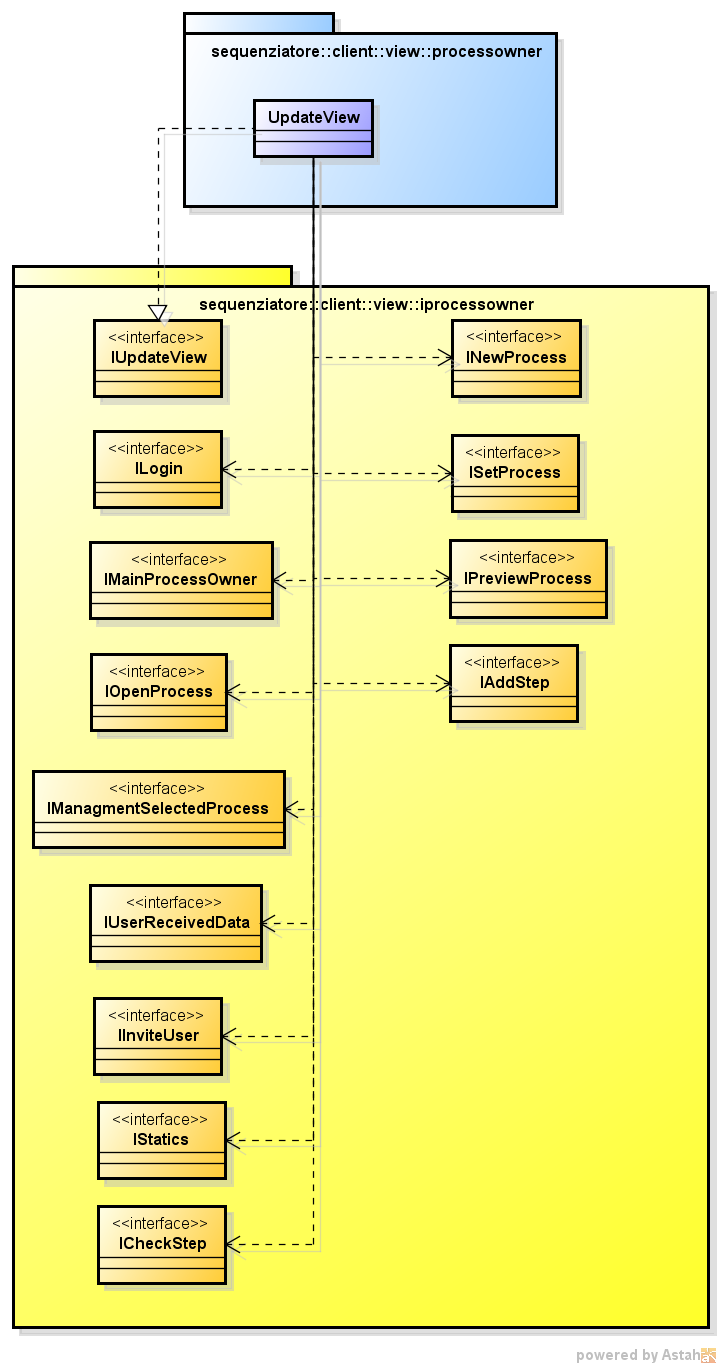
\includegraphics[scale=0.5]
{./pack/UpdateViewPo.png} \caption{Diagramma aggiornamento view process owner}
\end{figure}
\begin{itemize}
\item \textbf{Nome:} \texttt{IUpdateView};
\item \textbf{Package:} \texttt{\iViewAdmin{}};
\item \textbf{Descrizione:} Interfaccia che permette di gestire l'aggiornamento dei \textit{widget\ped{G}} della componente \textit{view}.
\end{itemize}

\paragraph{ILogin}
\begin{itemize}
\item \textbf{Nome:} \texttt{ILogin};
\item \textbf{Package:} \texttt{\iViewAdmin{}};
\item \textbf{Descrizione:} Interfaccia che permette di gestire l'interfaccia grafica relativa alle richieste di autenticazione e chiusura della sessione da parte dell'utente \textit{process owner\ped{G}}.
\end{itemize}

\paragraph{ISetProcess}
\begin{figure}[H] \centering 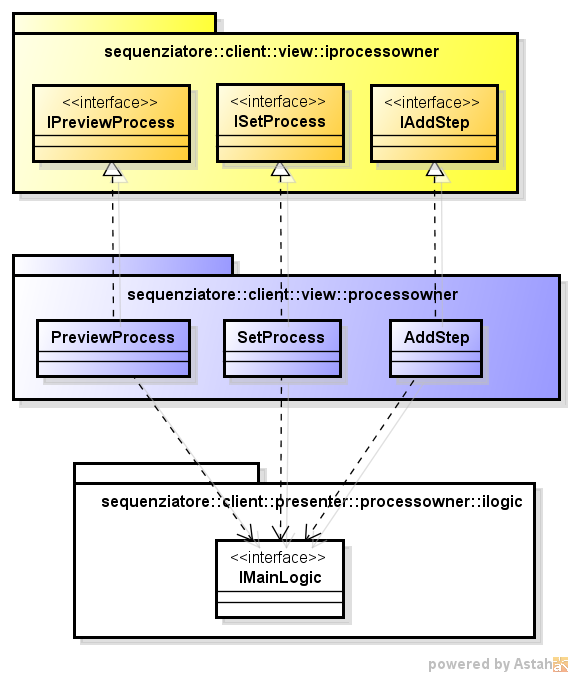
\includegraphics[width=%
\textwidth]
{./pack/newProcess.png} \caption{Diagramma view creazione nuovo processo}
\end{figure}
\begin{itemize}
\item \textbf{Nome:} \texttt{ISetProcess};
\item \textbf{Package:} \texttt{\iViewAdmin{}};
\item \textbf{Descrizione:} Interfaccia che permette di gestire l'interfaccia grafica che consente di creare nuovi processi.
\end{itemize}

\paragraph{IAddStep}
\begin{itemize}
\item \textbf{Nome:} \texttt{IAddStep};
\item \textbf{Package:} \texttt{\iViewAdmin{}};
\item \textbf{Descrizione:} Interfaccia che permette di gestire l'interfaccia grafica che consente di definire un nuovo passo del processo in creazione.
\end{itemize}

\paragraph{IPreviewProcess}
\begin{itemize}
\item \textbf{Nome:} \texttt{IPreviewProcess};
\item \textbf{Package:} \texttt{\iViewAdmin{}};
\item \textbf{Descrizione:} Interfaccia che permette realizzare i \textit{widget} che consentono di visualizzare l'anteprima del processo in creazione.
\end{itemize}

\paragraph{IOpenProcess}
\begin{itemize}
\item \textbf{Nome:} \texttt{IOpenProcess};
\item \textbf{Package:} \texttt{\iViewAdmin{}};
\item \textbf{Descrizione:} Interfaccia che permette di realizzare i \textit{widget} che consentono di aprire un processo tramite ricerca o selezione da una lista.
\end{itemize}

\paragraph{IManagmentSelectedProcess}
\begin{figure}[H] \centering 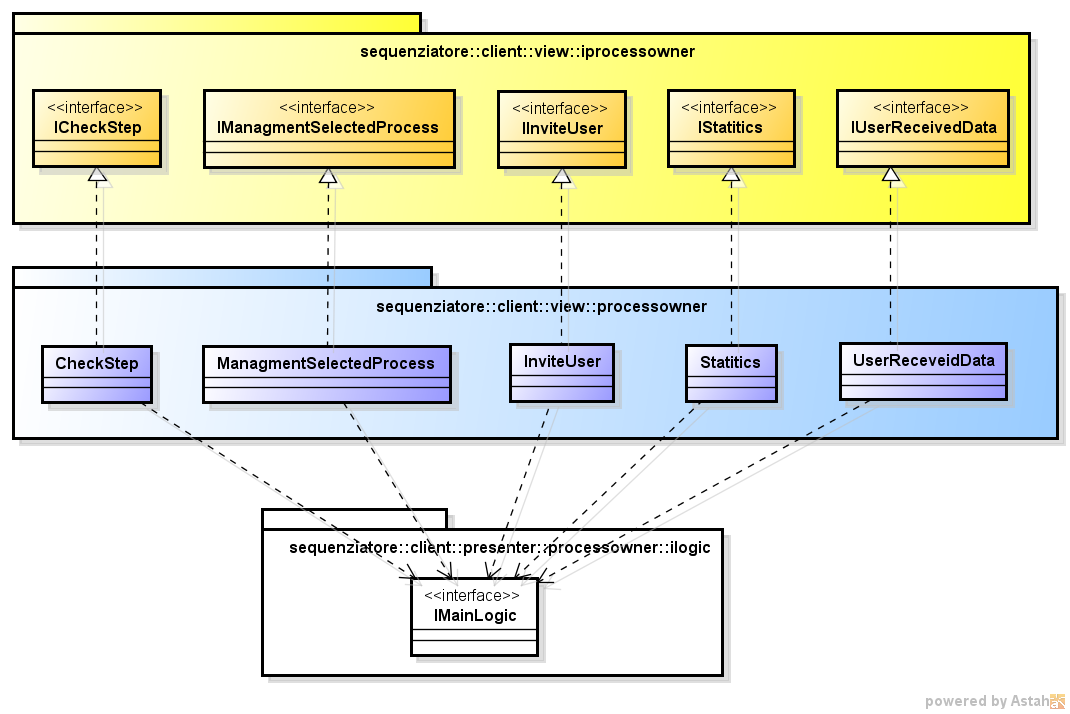
\includegraphics[width=%
\textwidth]
{./pack/PO_ManagmentSelectedProcess.png} \caption{Diagramma view gestione processi creati}
\end{figure}
\begin{itemize}
\item \textbf{Nome:} \texttt{IManagmentSelectedProcess};
\item \textbf{Package:} \texttt{\iViewAdmin{}};
\item \textbf{Descrizione:} Interfaccia che permette di realizzare i \textit{widget} che consentono di gestire i processi selezionati.
\end{itemize}

\paragraph{ICheckStep}
\begin{itemize}
\item \textbf{Nome:} \texttt{ICheckStep};
\item \textbf{Package:} \texttt{\iViewAdmin{}};
\item \textbf{Descrizione:} Interfaccia che permette di realizzare i \textit{widget} che consentono di gestire il controllo dei passi che richiedono intervento umano.
\end{itemize}

\paragraph{IStatistics}
\begin{itemize}
\item \textbf{Nome:} \texttt{IStatistics};
\item \textbf{Package:} \texttt{\iViewAdmin{}};
\item \textbf{Descrizione:} Interfaccia che permette di realizzare i \textit{widget} che consentono di gestire l'accesso alle informazioni statistiche sui processi.
\end{itemize}

\paragraph{IUserReceivedData}
\begin{itemize}
\item \textbf{Nome:} \texttt{IUserReceivedData};
\item \textbf{Package:} \texttt{\iViewAdmin{}};
\item \textbf{Descrizione:} Classe che permette di realizzare i \textit{widget} che consentono di gestire l'accesso ai dati inviati al \textit{server\ped{G}} dagli utenti;
\end{itemize}

\paragraph{IInviteUser}
\begin{itemize}
\item \textbf{Nome:} \texttt{IInviteUser};
\item \textbf{Package:} \texttt{\iViewAdmin{}};
\item \textbf{Descrizione:} Interfaccia che permette di realizzare i \textit{widget} che consentono di gestire i permessi di iscrizione ad un processo da parte degli utenti.
\end{itemize}